
\section{Methodology}
\begin{frame}[shrink=30]
    \frametitle{Methodology (1/2)}
    \begin{columns}
        \begin{column}{0.4\textwidth}
            \centering
            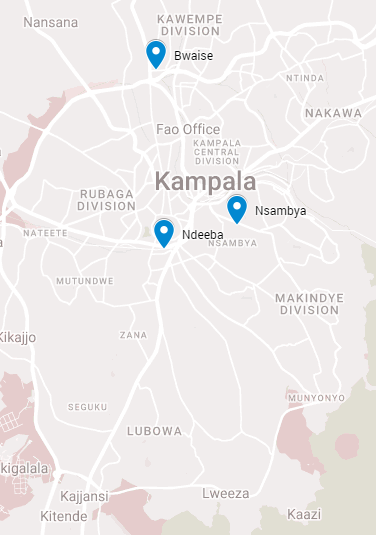
\includegraphics[width=\textwidth]{../../Common/figures/studyArea.png} % Replace with your image path
        \end{column}
        \begin{column}{0.6\textwidth}
            \textbf{1. Study Setting:} Kampala, Uganda
            \begin{itemize}
                \item 23\% urbanized, 60\% semi-urbanized, 17\% rural.
            \end{itemize}
            
            
            \textbf{3. Study Design:}
            \begin{itemize}
                \item Cross-sectional, quantitative.
            \end{itemize}
            
            \textbf{4. Sampling Technique:}
            \begin{itemize}
                \item Probability (random) and non-probability (purposive) sampling.
            \end{itemize}
            
            \textbf{5. Sampling Design:}
            \begin{itemize}
                \item Areas: 
            \end{itemize}
        \end{column}
    \end{columns}
\end{frame}
    
    
    


    \begin{frame}[shrink=20]
        \frametitle{Methodology (2/2)}
        \textbf{6. Sample Size Calculation:}
        \begin{itemize}
            \item Kish-Leslie formula: 50\% prevalence, 95\% confidence, 5\% margin of error.
        \end{itemize}
        
        \textbf{7. Data Collection:}
        \begin{itemize}
            \item Tools: Questionnaire, interviews, visual assessments.
            \item Pretest: 5 participants.
        \end{itemize}
        
        \textbf{8. Quality Control:}
        \begin{itemize}
            \item Pretesting tools, verifying data accuracy.
        \end{itemize}
        
        \textbf{9. Data Analysis:}
        \begin{itemize}
            \item Tools: Microsoft Excel for data summarization.
        \end{itemize}
        
        \textbf{10. Dissemination:}
        \begin{itemize}
            \item Reports to 
        \end{itemize}
\end{frame}
        
    


